\documentclass[utf8,a4paper,nofonts,9pt]{ctexbook}

\usepackage{amsmath}
\usepackage{xcolor}
\usepackage{hyperref}
\usepackage{graphicx}
\usepackage[many]{tcolorbox}
% \usepackage[left=0.65in, right=0.65in, top=0.95in, bottom=0.95in]{geometry}
\usepackage[inner=1in, outer=1.25in]{geometry}

\usepackage{src/package/Listings}

\NewDocumentCommand\TODO{m}{\footnote{\textcolor{red}{TODO: #1}}}

\def\dif{\mathop{}\!\mathrm{d}}

\newtcolorbox{exampleBox}{
    sharpish corners, % better drop shadow
    boxrule = 0pt,
    toprule = 4.5pt, % top rule weight
    enhanced,
    fuzzy shadow = {0pt}{-2pt}{-0.5pt}{0.5pt}{black!35} % {xshift}{yshift}{offset}{step}{options} 
}

\setCJKmainfont[Path=../fonts/,BoldFont=SourceHanSerifCN-Bold.otf,ItalicFont=SourceHanSerifCN-Bold.otf]{SourceHanSerifCN-Regular.otf}
\setCJKsansfont[Path=../fonts/,BoldFont=SourceHanSansCN-Bold.otf]{SourceHanSansCN-Regular.otf}
\setCJKmonofont[Path=../fonts/]{SourceHanSansCN-Regular.otf}

\title{Cookbook}
\author{周泓余\thanks{PeterlitsZo}}

\begin{document}

\maketitle

\tableofcontents
\newpage

\chapter{数学}

虽然我的确想要把所有笔记都记录在 Obsidian 中,但是数学相关的内容用 Obsidian 写起来还是太麻烦了。还是挪到这里吧。

\section{统计和概率学}

\subsection{正态分布}

我们说一个随机变量 $X$ 服从正态分布,那么我们记为 $X \sim N(\mu, \sigma^2)$。

这里的 $\mu$ 表示期望,$\sigma^2$ 表示方差。正态分布的概率密度函数为:

$$
f(x) = {1 \over \sqrt{2\pi}\sigma} \exp\left(-{(x - \mu)^2 \over 2\sigma^2}\right)
$$

我们将 $X \sim N(0, 1)$ 的随机变量称为标准正态分布。这个时候我们带入有概率密度函数如下:

$$
f(x) = {1 \over \sqrt{2\pi}} \exp\left(-{x^2 \over 2}\right)
$$

另外,对于 $X \sim N(\mu, \sigma^2)$ 而言,我们可以说 $Y = {X - \mu \over \sigma}$ 服从标准正态分布。

在 Rust 中,我们可以通过下面的方式来完成模拟(这里的 \verb|v| 即为一个正态分布的抽样):

\begin{lstlisting}
use rand_distr::{Distribution, Normal};

let normal = Normal::new(0.0, 1.0).unwrap();
let v = normal.sample(&mut rand::rng());
println!("{} is from a N(0, 1) distribution", v);
// 0.8033917292233297 is from a N(0, 1) distribution
\end{lstlisting}

在文档项目中的 \verb|playground| 目录下运行下面的命令即可:

\begin{lstlisting}
cargo run --bin 00_normal
\end{lstlisting}

\subsection{伊藤引理}
\label{title:ItosLemma}

[TODO]

\subsection{标准布朗运动}

我们这么定义标准布朗运动,对于定义在非负实数(时域)$t$ 上的连续随机过程 $\{B_t, t \ge 0\}$,满足以下条件:

\begin{itemize}
    \item $B(0) = 0$;
    \item 平稳性:对于所有 $0 < s < t$,增量 $B(t) - B(s)$ 符合均值为 $0$,方差为 $t - s$ 的正态分布。
    \item 独立增量:对于所有 $0 \le s < t < u < v$,增量 $B(t) - B(s)$ 和 $B(v) - B(u)$ 是独立的。
\end{itemize}

这个时候我们就说 $B(t)$ 是一个标准布朗运动。

在编程实现中,想要模拟连续的标准布朗运动是不现实且没有必要的,我们可以用离散的方式来模拟。
在 Rust 中,随机数可以通过 \verb|rand| 来生成,但是为了通过正态分布生成随机数,我们还需要使用 \verb|rand_distr|。
我们假设按照单位时间为 1s,那么中国股市的一天的交易时间就一共有 14400 个单位时间(对应 4 个小时)。
我们尝试循环 14400 次,每次都生成单位时间内对应的差 $\Delta B$,并且将其累加到 $B$ 上。
根据标准布朗运动的定义,我们很容易知道 $\Delta B$ 服从一个均值为 0,方差为 1 的标准正态分布(我们定义单位时间的长度就是 $1$)。
然后因为增量都是独立的,所以 $\Delta B$ 的求值和之前的求值无关,这是一个非常优良的特征。这使得下面的代码很容易实现:

\begin{lstlisting}
use rand_distr::{Distribution, Normal};

fn std_brownian_motion(steps: usize) -> Vec<f64> {
    let mut rng = rand::rng();

    let normal = Normal::new(0.0, 1.0).unwrap();
    let mut bm = vec![0.0];

    for _ in 0..steps {
        let v = normal.sample(&mut rng);
        bm.push(bm.last().unwrap() + v);
    }

    bm
}

std_brownian_motion(14400);
\end{lstlisting}

在文档项目中的 \verb|playground| 目录下运行如下命令即可:

\begin{lstlisting}
cargo run --bin 01_std_brownian_motion
\end{lstlisting}

在浏览器中,可以看到标准布朗运动的图像。如图 \ref{fig:stdBrownianMotion} 所示。

\begin{figure}[h]
    \centering
    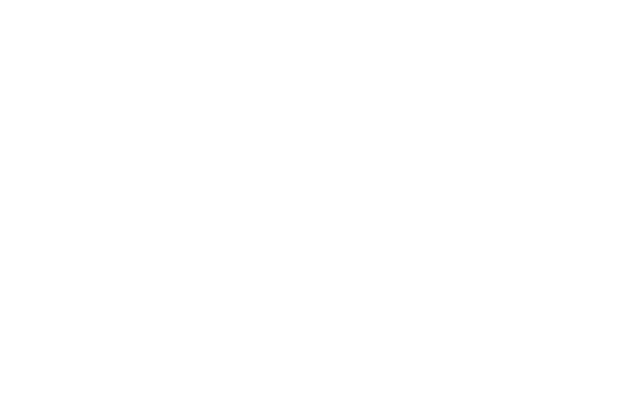
\includegraphics[width=0.8\textwidth]{src/static/00_std_brownian_motion.png}
    \caption{标准布朗运动}
    \label{fig:stdBrownianMotion}
\end{figure}

\subsection[几何布朗运动]{几何布朗运动\protect\footnotemark}
\footnotetext{见 \url{https://zhuanlan.zhihu.com/p/38293827}。}

我们可以在标准布朗运动 $B(t)$ 的基础上定义几何布朗运动。在定义之前,我们先定义有漂移的布朗运动 $X(t)$,它有:

$$
\dif{X(t)} = \mu \dif{t} + \sigma \dif{B(t)}
$$

我们知道 $B(t)$ 随机变量在 $t = 1$ 的期望为 $0$,而标准差为 $1$,经过偏移后,$X(t)$ 的期望和方差属性都有所变化。
这里 $\mu$ 被用于表示在单位时间内的期望增长率,而 $\sigma$ 被用于表示单位时间内的标准差。

在量化交易中,我们可以使用这个来描述收益率,而对于股票价格 $S(t)$ 而言,因为有 ${\dif{S(t)} \over S(t)} = \dif{X(t)}$。所以有:

$$
\dif{S(t)} = \mu S(t) \dif{t} + \sigma S(t) \dif{B(t)}
$$

通过伊藤引理 \ref{title:ItosLemma},我们可以得到:

$$
S(t) = S_0 \exp\left(\left(\mu - {\sigma^2 \over 2}\right)t + \sigma B(t)\right)
$$

我们可以使用 Rust 来对齐进行描述:

\begin{lstlisting}
use rand_distr::{Distribution, Normal};

fn geo_brownian_motion(steps: usize, mu: f64, sigma: f64, s0: f64) -> Vec<f64> {
    let mut rng = rand::rng();

    let normal = Normal::new(0.0, 1.0).unwrap();
    let mut bm = vec![s0];

    for _ in 0..steps {
        let z = normal.sample(&mut rng);
        let last_val = bm.last().unwrap();

        let drift = mu - 0.5 * sigma.powi(2);
        let diffusion = sigma * z;
        let new_val = last_val * (drift + diffusion).exp();

        bm.push(new_val);
    }

    bm
}
\end{lstlisting}

在 \verb|playground| 目录下运行如下命令即可:

\begin{lstlisting}
cargo run --bin 02_geo_brownian_motion
\end{lstlisting}

可以在浏览器中看到对应的几何布朗运动的图像。图 \ref{fig:geoBrownianMotion} 展示了几何布朗运动的一个例子。
(在这个图中,我们假定它为一个指数的日内曲线,其中年化收益率为 $8\%$,而一年的方差设置为 $10$)。

\begin{figure}[h]
    \centering
    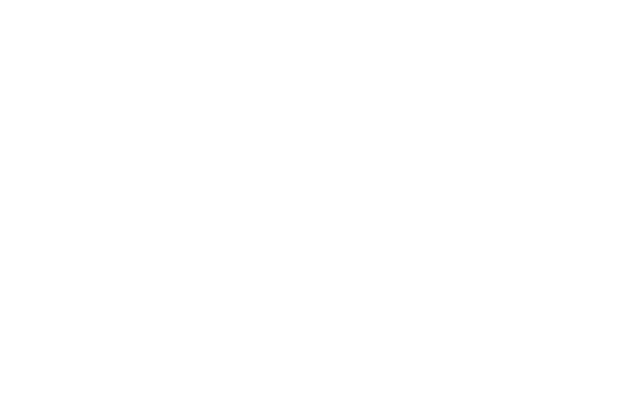
\includegraphics[width=0.8\textwidth]{src/static/01_geo_brownian_motion.png}
    \caption{几何布朗运动}
    \label{fig:geoBrownianMotion}
\end{figure}

\chapter{金融经济学}

\section{标的属性}

\subsection{股票市盈率}

市盈率是市价盈利比率(price earnings ratio,P/E)的简称。

我们在 \ref{title:DDM} 节中讨论了 DDM 模型,它指出了股票的价格取决于其预期分红。而企业往往在盈利后才会有分红。
所以为了给股票估值,那么我们往往会研究这个股票估值指标,即市盈率。它的值是股票价格和每股盈利的比值。
而每股盈利则是公司总盈利除以公司的总股份数。

注意到公司不会将所有盈利都用来分红,公司往往会将一部分盈利拿来用以分红,那么将这个比例记为 $k$,第 $t$ 期的每股分红 $D_t$ 和每股盈利 $E_t$ 有

$$
E_t = kD_t
$$

将其带入到 \ref{title:DDM} 节中的戈登股利增长模型中有

$$
{S_0 \over E_1} = {k \over r - g}
$$

这里的左式即为市盈率。即市盈率取决于分红率、贴现率和盈利增速这三个变量。

这说明了即使一个企业的每股盈利较高,但是如果企业以较低分红率分红的话,投资者也不会愿意投资这个企业。
同样,盈利增速也是一个非常重要的因素,它即使发生的是一点点变化,也会大幅度影响 P/E 的值。

\begin{exampleBox}
如果我们说一个股票的 P/E 为 10,而每股盈利为 10 元的话,那么可以说这个公司的股价在理论上应该为 100 元。
如果我们说因为某种原因,导致了预期的盈利增速 $g$ 发生了变化(比如政策倾斜),即使这个公司在短期内每股盈利不变,但是也会导致市盈率大幅上涨,从而导致价格也大幅上涨。
比如如果 $r = 20\%$,而 $g = 16\%$ 上涨到了 $g' = 18\%$,这个 $2\%$ 的上涨会导致 P/E 翻倍,最后导致股票价格也翻倍。
\end{exampleBox}

\begin{exampleBox}
和上一个例子一样,我们假设 $S_0 = 100$,$E_1 = 10$,$k = 40\%$,$g = 16\%$ 以及 $r = 20\%$,我们来计算投资者在第 0 期买入,到第 1 期卖出得到的回报率。
可以知道投资回报率为

$$
{D_1 + S_1 \over S_0} - 1
$$

即一期得到的分红以及股票价格之和相比一开始的股票价格的涨幅。
我们知道 $D_1 = k E_1 = 4$,而 $S_1 = {D_2 \over r - g} = {D_1 (1 + g) \over r - g} = 116$,所以有

$$
{4 + 116 \over 100} - 1 = 20\% = r
$$

可以知道市场的投资回报率为 $r = 20\%$。这个不难证明。所以贴现率即为投资者所能接受且理论上能获得的回报率(如果实际产生的回报率高于贴现率,那么对这个股票的需求就会上涨,导致价格上涨,进而拉低回报率,最后达到均衡)。
\end{exampleBox}

在实践中,我们一般使用滚动市盈率(trailing P/E)来表示市盈率,即市盈率 TTM,其中 TTM 表示 trailing twelve months,即根据过去的 12 个月来计算出来的市盈率。
在实践中上市公司会一年发布四次财报,所以实践中我们会用过去 4 个财报的盈利数字之和作为市盈率的分母
\footnote{理论上来说,市盈率应该使用未来一年的盈利来作为分母,但是很可惜截止目前还没有会时空穿越的金融奇才。},所以和市盈率 P/E 表示的 $S_0 / E_1$ 不同,P/E TTM 表示的是 $S_0 / E_0$。
而对于高成长的公司,往往 $E_1$ 和 $E_0$ 之间的差距较大,这个时候我们需要预测未来的十二个月的盈利。我们使用预测的盈利来计算市盈率,这个时候我们就得到了前瞻市盈率(forward P/E)。

除了市盈率,我们还有市净率(price to book ratio,P/B)等指标,表示每股股价和每股净资产。

\section{金融模型和理论}

\subsection{股利贴现模型}
\label{title:DDM}

股利贴现模型(dividend discount model),也就是 DDM,可以用如下的表达式来完成表达

$$
S_0 = {D_1 + S_1 \over 1 + r} = \sum_{t=1}^{\infty} {D_t \over (1 + r)^t} + \lim_{t \to \infty} {P_t \over (1 + r)^t}
$$

这里的 $S_t$ 即表示在 $t$ 期时候的价格,而 $r$ 表示贴现率,而 $D_t$ 表示在 $t$ 期时候的分红。
可以看到,因为我们假设市场是无套利的,所以当前股票的价格理论上应该是分红和除红利价格之和,除以 $1 + r$ 之后的价格。
将这个过程无限延伸下去,我们就可以得到上面的公式。

我们对其设置一个截断性条件,即

$$
\lim_{t \to \infty} {P_t \over (1 + r)^t} = 0
$$

那么有

$$
S_0 = \sum_{t=1}^{\infty} {D_t \over (1 + r)^t}
$$

而我们为了简单起见,可以假设 $D_t = D_0 (1 + g)^t$,那么有

$$
S_0 = {D_1 \over r - g}
$$

这个方程被称为戈登模型。

\subsection{均值-方差模型}
\label{title:E-sigma-model}

在金融资产这个主题中,债卷,尤其是国债,是一种如果我们在当前买入,就一定能知道未来能得到多少收益的金融资产。对于这种未来收益给定了的资产,和股票等金融资产不同,我们可以说它的基本没有所谓的 “不确定性”。我们可以使用波动性来量化金融资产未来价格的 “不确定性”,即我们可以说国债的波动率是 0。

但是对于其他具有这种 “不确定性” 的金融资产而言,比如股票,该资产的波动率是无法计算的(也就是说,如果我们当前买入了该资产,并持有一个时期之后,这个资产对应的回报率对应的概率密度函数是无法确定的)。

但是在实际中,我们假设资产的回报率对应的概率密度函数是大体不变的,这使得我们可以通过从历史的价格走势来估计未来价格的概率密度函数,进一步的,从过去价格走势我们能计算出(或者说估算出)当前金融资产的波动率,同样地也能计算出预期收益。这样我们能对某个金融资产计算出对应的回报率的均值和方差。有均值

$$
\bar{r} = {1 \over N}\sum_{i = 1}^{N} r_i
$$

这里我们回顾历史 $N$ 个时期,每个时期的回报率 $r_i$ 是能够获取的,这个时候这个资产的均值 $\bar{r}$ 能够通过上式来完成计算,它的金融含义即为预期的回报率。回报率的方差可以通过下式来完成计算。

$$
\sigma_r^2 = {1 \over N}\sum_{i = 1}^{N} \left( r_i - \bar{r} \right)^2
$$

方差的算术平方根,即 $\sigma_r$,即为标准差,也为之前我们讨论的波动率。

资产和资产之间也互相有联系。比如如果两个互联网企业中某个互联网企业股价上涨了,另外一个互联网企业上涨的概率也会大一些。我们使用协方差来进行描述它们之间的相关程度。我们定义这两个企业的在历史第 $i$ 个时期的回报率分别是 $x_i$ 和 $y_i$,那么有

$$
\sigma_{xy} = {1 \over N} \sum_{i = 1}^{N} (x_i - \bar{x}) (y_i - \bar{y})
$$

将协方差 $\sigma_{xy}$ 标准化为相关系数 $\rho_{xy}$,有

$$
\rho_{xy} = {\sigma_{xy} \over \sigma_x \sigma_y}
$$

相关系数 $\rho_{xy}$ 在的取值范围为 $-1$ 到 $+1$。如果是 $+1$,我们称其为完全正相关,如果为 $-1$,我们称其为完全负相关。

考虑无风险资产和有风险资产的资产组合。无风险资产的回报率均值为 $\bar{r}_f$,标准差为 $0$,占比 $1 - \omega$。有风险资产的回报率均值为 $\bar{r_s}$,标准差为 $\sigma_s$,占比 $\omega$。容易证得它们的协方差为 $0$。那么组合的均值和方差有
\begin{align*}
    \bar{r}_p  & = (1 - \omega) \bar{r}_f + \omega \bar{r}_s = \bar{r}_f + \omega(\bar{r}_s - \bar{r}_f) \\
    \sigma_p^2 & = E\left[ (1 - \omega) r_f + \omega r_s - (1 - \omega) \bar{r}_f - \omega \bar{r}_s \right]^2 = E\left[ \omega^2 (r_s - \bar{r}_s)^2 \right] = \omega^2 \sigma_s^2
\end{align*}
这里的组合均值是通过方差的定义计算出来的。因为 $\omega = \sigma_p / \sigma_s$,那么有
\[
    \bar{r}_p = \bar{r}_f + {\bar{r}_s - \bar{r}_f \over \sigma_s} \sigma_p
\]
可以看到,如果 $\bar{r}_f > \bar{r}_s$,那么我们如果接收的组合波动率越大,我们的组合的收益期望也会跟着增大。

考虑两个有风险资产的资产组合,令回报率对应随机变量为 $r_1$ 和 $r_2$,它们的均值记为 $\bar{r}_1$ 和 $\bar{r}_2$,而标准差记为 $\sigma_1$ 和 $\sigma_2$,协方差记为 $\sigma{12}$。投在这两个资产的份额为 $\omega$ 和 $1 - \omega$,那么组合的回报率期望 $\bar{r}_p$ 满足
\[
    \bar{r}_p = \omega \bar{r}_1 + (1 - \omega) \bar{r}_2
\]
而回报率方差 $\sigma^2_p$ 为
\begin{align*}
    \sigma^2_p & = E\left[ \omega r_1 + (1 - \omega) r_2 - \omega \bar{r}_1 - (1 - \omega) \bar{r}_2 \right]^2 \\
               & = E\left[ \omega (r_1 - \bar{r}_1) + (1 - \omega) (r_2 - \bar{r}_2) \right]^2 \\
               & = E\left[ \omega^2 (r_1 - \bar{r}_1)^2 + (1 - \omega)^2 (r_2 - \bar{r}_2)^2 + 2 \omega (1 - \omega) (r_1 - \bar{r}_1) (r_2 - \bar{r}_2) \right] \\
               & = \omega^2 \sigma_1^2 + (1 - \omega)^2 \sigma_2^2 + 2 \omega (1 - \omega) \sigma_{12}
\end{align*}

因为有
\[
    \omega = {\bar{r}_p - \bar{r}_2 \over \bar{r}_1 - \bar{r}_2}
\]
那么我们可以将这个带入 $\sigma^2_p$ 对应的等式中,以消除 $\omega$,得到的等式有两个变量,即组合回报率期望 $\bar{r}_p$ 和组合回报率方差 $\sigma^2_p$。那么组合在期望-标准差坐标系中得到的对应曲线即为一个双曲线\footnote{我自己没有推导出来。}。

求偏导\footnote{因为不太会,所以没有自己推。},能够发现当 $\omega$ 为下时资产组合的方差最小
\[
    \omega^* = {\sigma_2^2 - \sigma_{12} \over \sigma_1^2 + \sigma_2^2 - 2 \sigma_{12}}
\]

这个结论告诉我们,如果我们分散化投资的话,我们可以在最小化方差的情况下取得一个还不错的期望。

考虑多个有风险资产的资产组合,资产组合在期望-标准差坐标系中就不再是一个曲线了,而是一个区域。这里有一个结论:在均值-标准差坐标系上,多种风险资产形成的组合区域边界是开口向右、上下对称的双曲线。这个双曲线的上半边被称为组合的有效前沿。

前文指出,多个有风险资产的资产组合在期望-标准差坐标系中构成来一个区域,其中交易者会关注这个资产组合的有效前言。而在前文我们又指出,有风险资产和无风险资产的资产组合能够在期望-标准差坐标系中构成一个射线(如果不允许买空的话,那么实际上应该是一个线段,但是如果允许买空的话,我们可以使用无风险资产的利率来借贷并买入有风险资产)。我们让这个射线和多个有风险资产的资产组合在期望-标准差坐标系中构成的区域相切,那么这个射线即为包含无风险资产的组合有效前沿,在金融学中被称为\emph{资本市场线}(简称
CML)。而资产市场线与双曲线的切点就是\emph{市场组合},一般使用字母 $M$ 表示。

市场组合 $M$ 的期望回报率为 $\bar{r}_M$,波动率为 $\sigma_M$,那么资本市场线的公式为
\[
    \bar{r} - \bar{r}_f = {\sigma \over \sigma_M} (\bar{r}_M - \bar{r}_f)
\]

这说明了一个事情,即理性的投资者,无论其偏好如何,他总是会使用市场组合的形式来持有有风险资产。投资者的风险偏好只会影响他们分配在无风险资产和市场组合的比例上。


\section{参考书目}

\begin{itemize}
    \item 《金融经济学二十五讲》,徐高,中国人民大学出版社;
\end{itemize}

\end{document}